% CHAPTER 4

\chapter{Results and Discussion}
\label{chap:results}


% 4.1 HYDROGEN BENCHMARK


\section{Hydrogen Benchmark}

The reference hydrogen calculation provides an initial assessment of how accurately the Gaussian
expansion reproduces the exact ground state. Using the parameters in Eq.~\eqref{eq:reference_parameters}, the calculated energy is $-0.4995891522$ Hartree, compared with
the exact value of $-0.5$ Hartree. The relative energy error is $8.2170\times10^{-4}$, or
approximately $0.0822\%$. The calculated energy lies above the exact value, as required by the
variational principle. The calculated mean radius is $1.50124491$ bohr, compared with the exact value of $1.5$ bohr. This corresponds to a relative radius error of approximately $8.30\times10^{-4}$, or $0.0830\%$. The
close agreement in both quantities suggests that the reference basis represents the overall
ground-state distribution well, although neither measure establishes its accuracy at every radius.

Table~\ref{tab:hydrogen_benchmark} summarises the benchmark results. The overlap condition number of
$8.3295\times10^4$ also provides a reference for the conditioning behaviour examined later.

\begin{table}[htbp]
\centering
\caption{Hydrogen ground-state benchmark for
$N=12$, $\alpha=0.01\,\mathrm{bohr}^{-2}$ and $\beta=1.9$.
Exact reference values are obtained from the analytical
hydrogenic ground-state solution in Section~2.1
for $Z=1$.}
\label{tab:hydrogen_benchmark}
\begin{tabular}{lcc}
\hline
Quantity & Exact & Gaussian basis\\
\hline
Energy (Hartree)
    & $-0.500000$ & $-0.499589$\\
Mean radius (bohr)
    & $1.500000$ & $1.501245$\\
Relative energy error
    & $0$ & $8.2170\times10^{-4}$\\
Overlap condition number
    & --- & $8.3295\times10^4$\\
\hline
\end{tabular}
\end{table}

\begin{figure}[htbp]
\centering
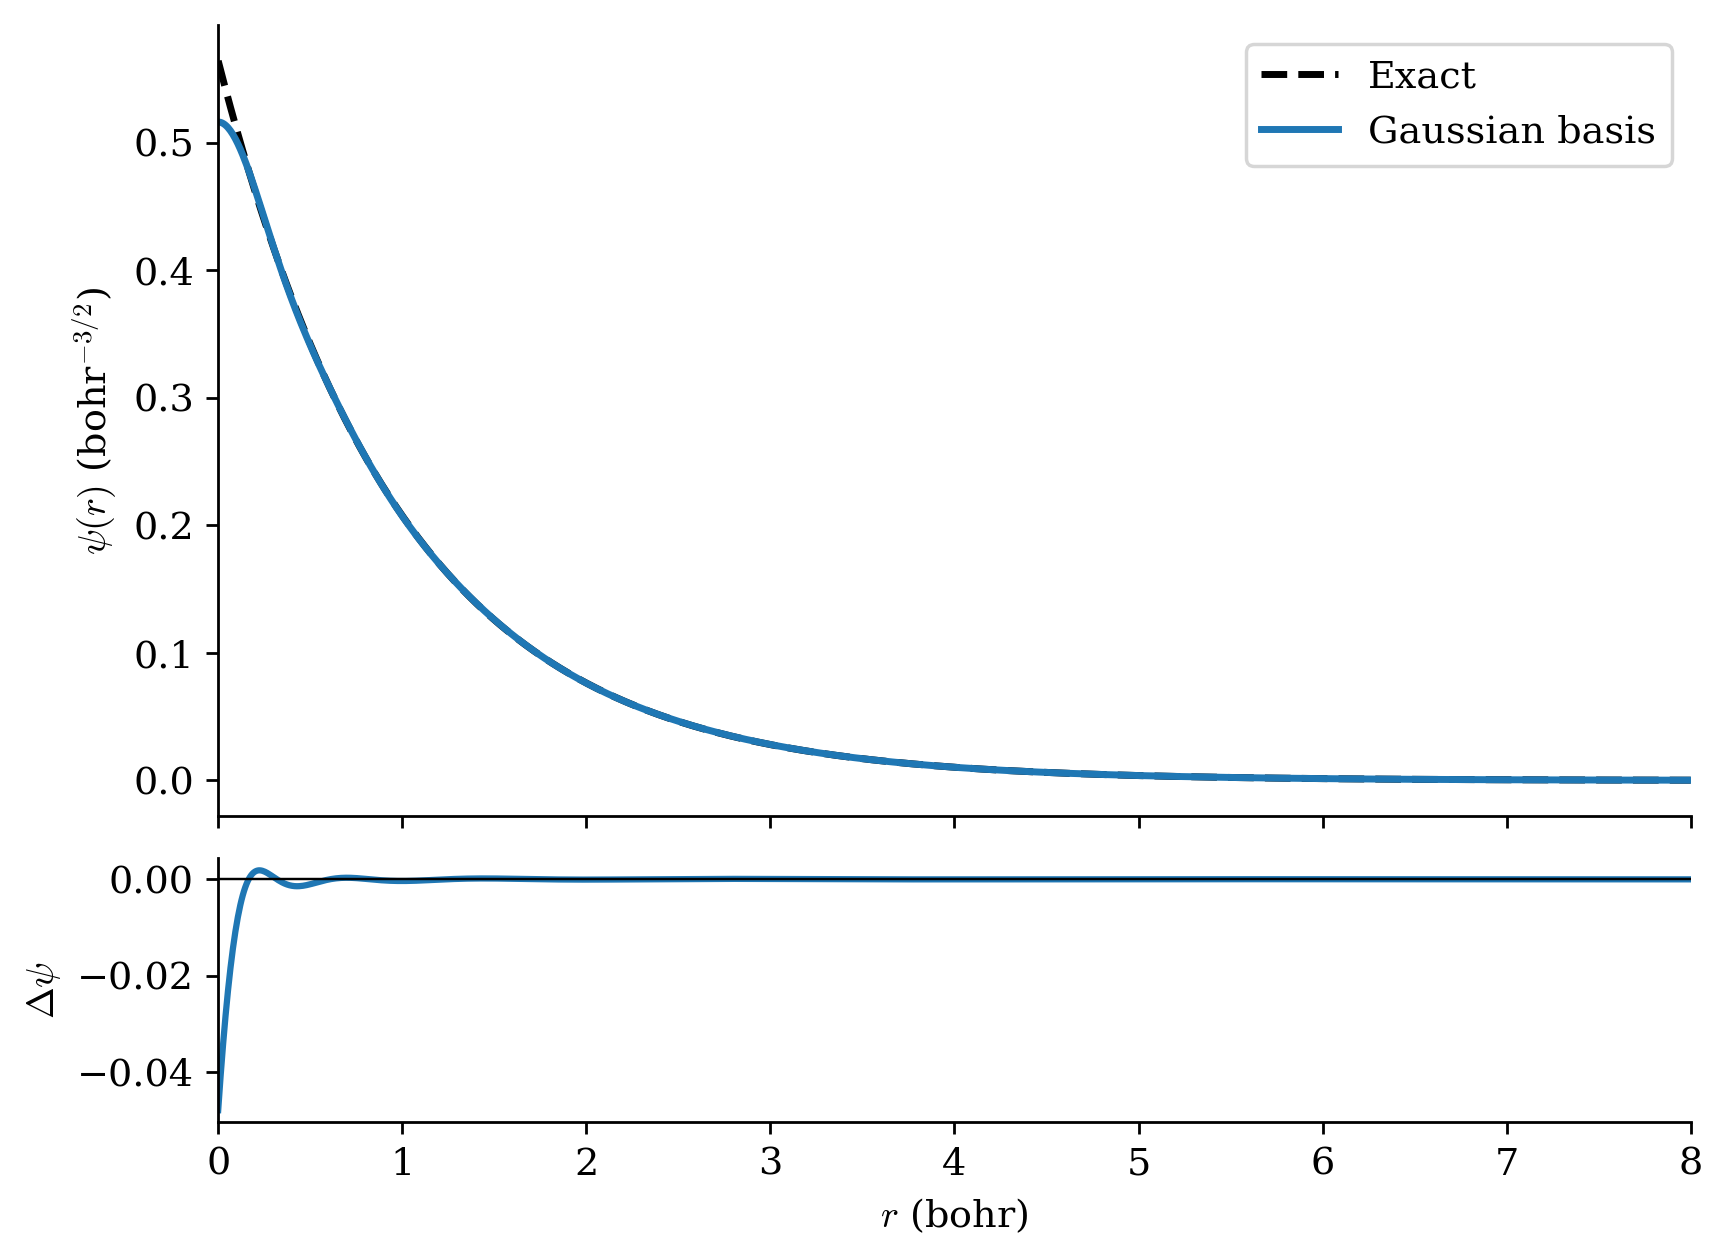
\includegraphics[width=0.82\linewidth]
{Figures/01_hydrogen_wavefunction.png}
\caption{Exact and Gaussian hydrogen ground-state
wavefunctions, together with their signed difference.
The discrepancy is most apparent near the nucleus,
despite close agreement over most of the radial range.}
\label{fig:hydrogen_wavefunction}
\end{figure}

Figure~\ref{fig:hydrogen_wavefunction} compares the exact and approximate wavefunctions directly.
Their overall shapes agree closely, but the signed difference reveals a more noticeable discrepancy
near the nucleus.
At $r=0$, the Gaussian expansion gives
$\psi_{\mathrm G}(0)=0.516211566\
\mathrm{bohr}^{-3/2}$, compared with
$\psi_{1s}(0)=0.564189584\
\mathrm{bohr}^{-3/2}$.
The relative amplitude difference is:
\[
    \frac{|\psi_{\mathrm G}(0)-\psi_{1s}(0)|}
         {|\psi_{1s}(0)|}
    \approx 0.0850,
\]
corresponding to an underestimate of approximately
$8.5\%$.

The electron density depends on the square of the
wavefunction amplitude. The corresponding relative
density difference at the nucleus is:
\[
    1-\frac{|\psi_{\mathrm G}(0)|^2}
            {|\psi_{1s}(0)|^2}
    \approx 0.163,
\]
or approximately $16.3\%$. These local errors are substantially larger than the $0.0822\%$ energy error. The variational energy therefore gives a favourable assessment of the reference basis that is not representative of its
accuracy at the nucleus. This matters for physical quantities that depend strongly on the electron
density or wavefunction behaviour in the near-nuclear region.

\begin{figure}[htbp]
\centering
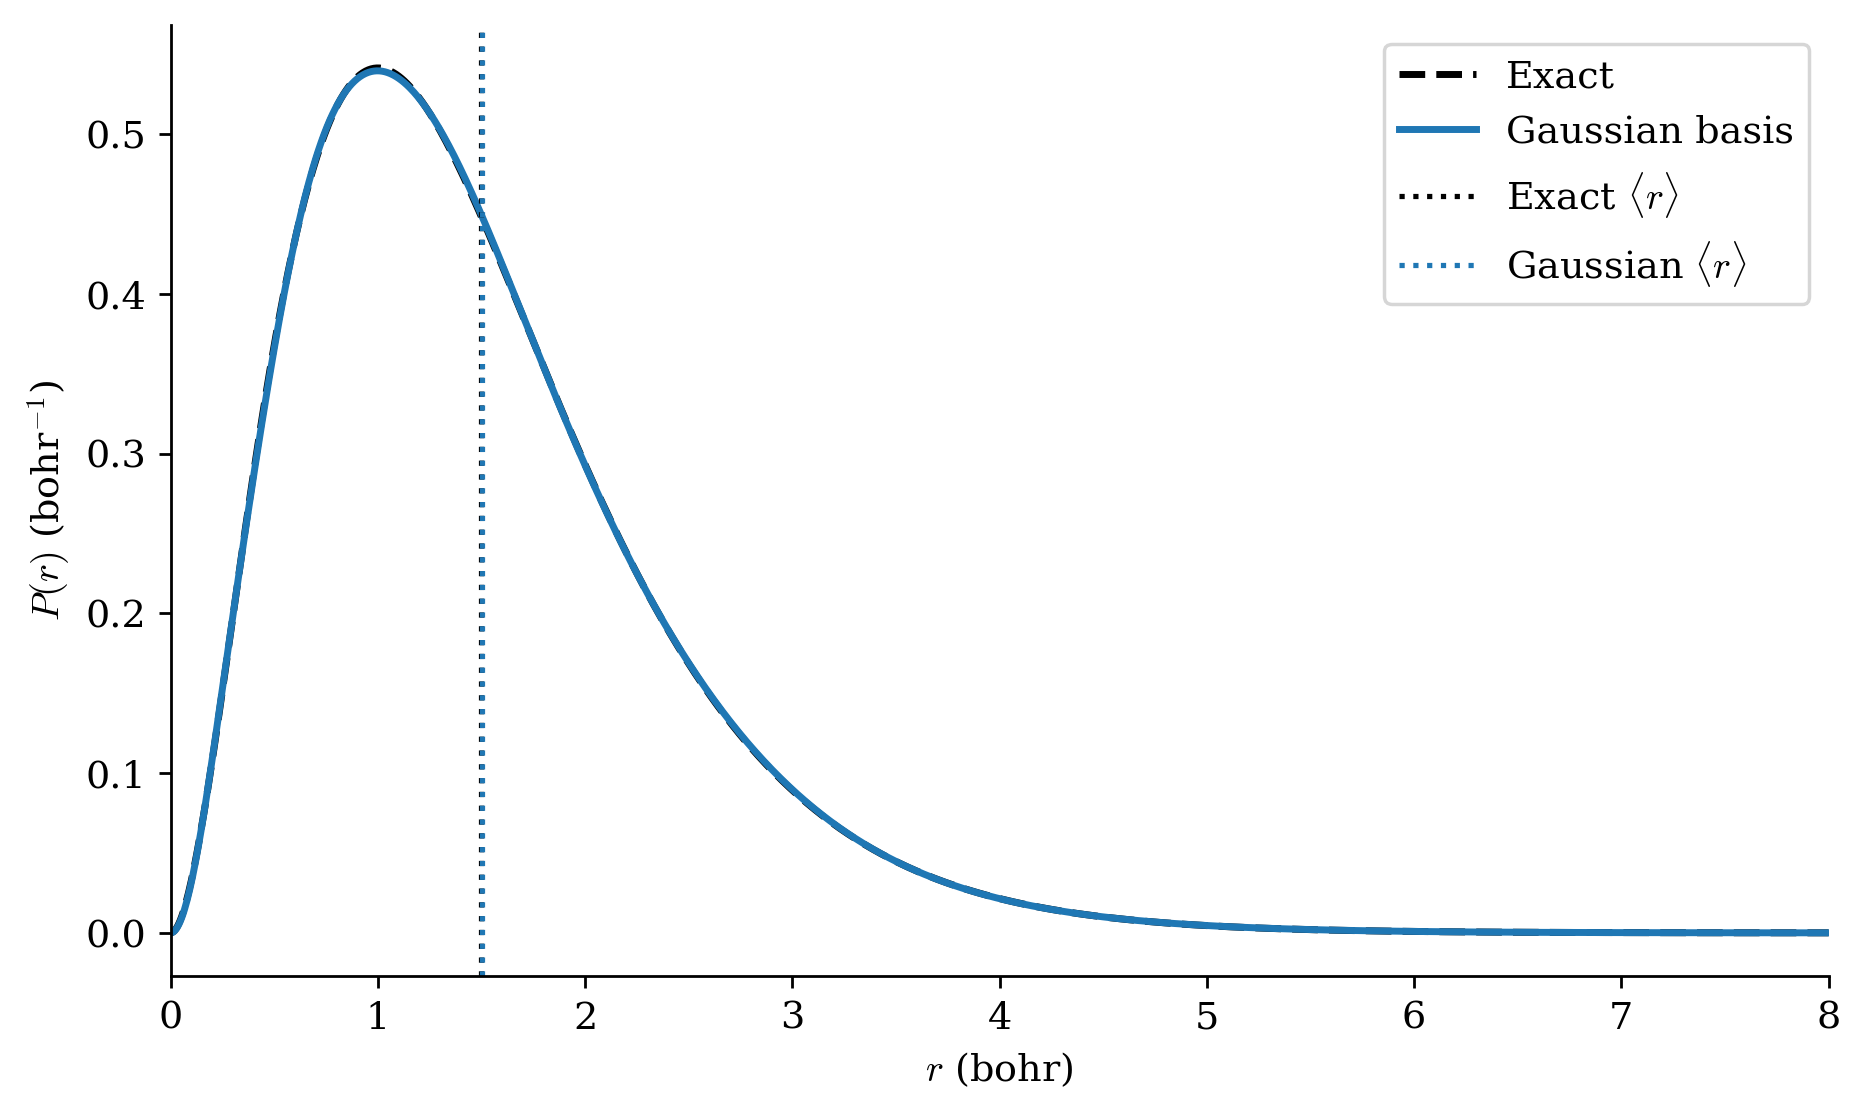
\includegraphics[width=0.82\linewidth]
{Figures/02_hydrogen_radial_probability.png}
\caption{Exact and Gaussian radial probability
distributions for hydrogen, with their mean radii
indicated. The mean radius is distinct from the
position of maximum radial probability.}
\label{fig:hydrogen_radial}
\end{figure}

The radial probability distributions in Fig.~\ref{fig:hydrogen_radial} show even closer agreement.
The radial probability density contains the factor $4\pi r^2$, which suppresses the contribution
from the immediate vicinity of the nucleus. Consequently, the distributions can appear nearly identical despite the appreciable difference between the wavefunction amplitudes at $r=0$.
This also helps explain why the mean radius is reproduced accurately. The expectation value $\langle
r\rangle$ depends on the entire radial distribution, with additional weighting towards larger radii,
rather than on the wavefunction at a single point.
The benchmark therefore reveals two aspects of the approximation. The Gaussian expansion captures
the overall ground-state energy and radial distribution well, but its local accuracy is considerably
poorer near the nucleus. This difference motivates the separate convergence and near-nuclear tests
that follow.


% 4.2 BASIS-SIZE CONVERGENCE AND EXPONENT SELECTION


\section{Basis-Size Convergence and Exponent Selection}

\begin{figure}[htbp]
\centering
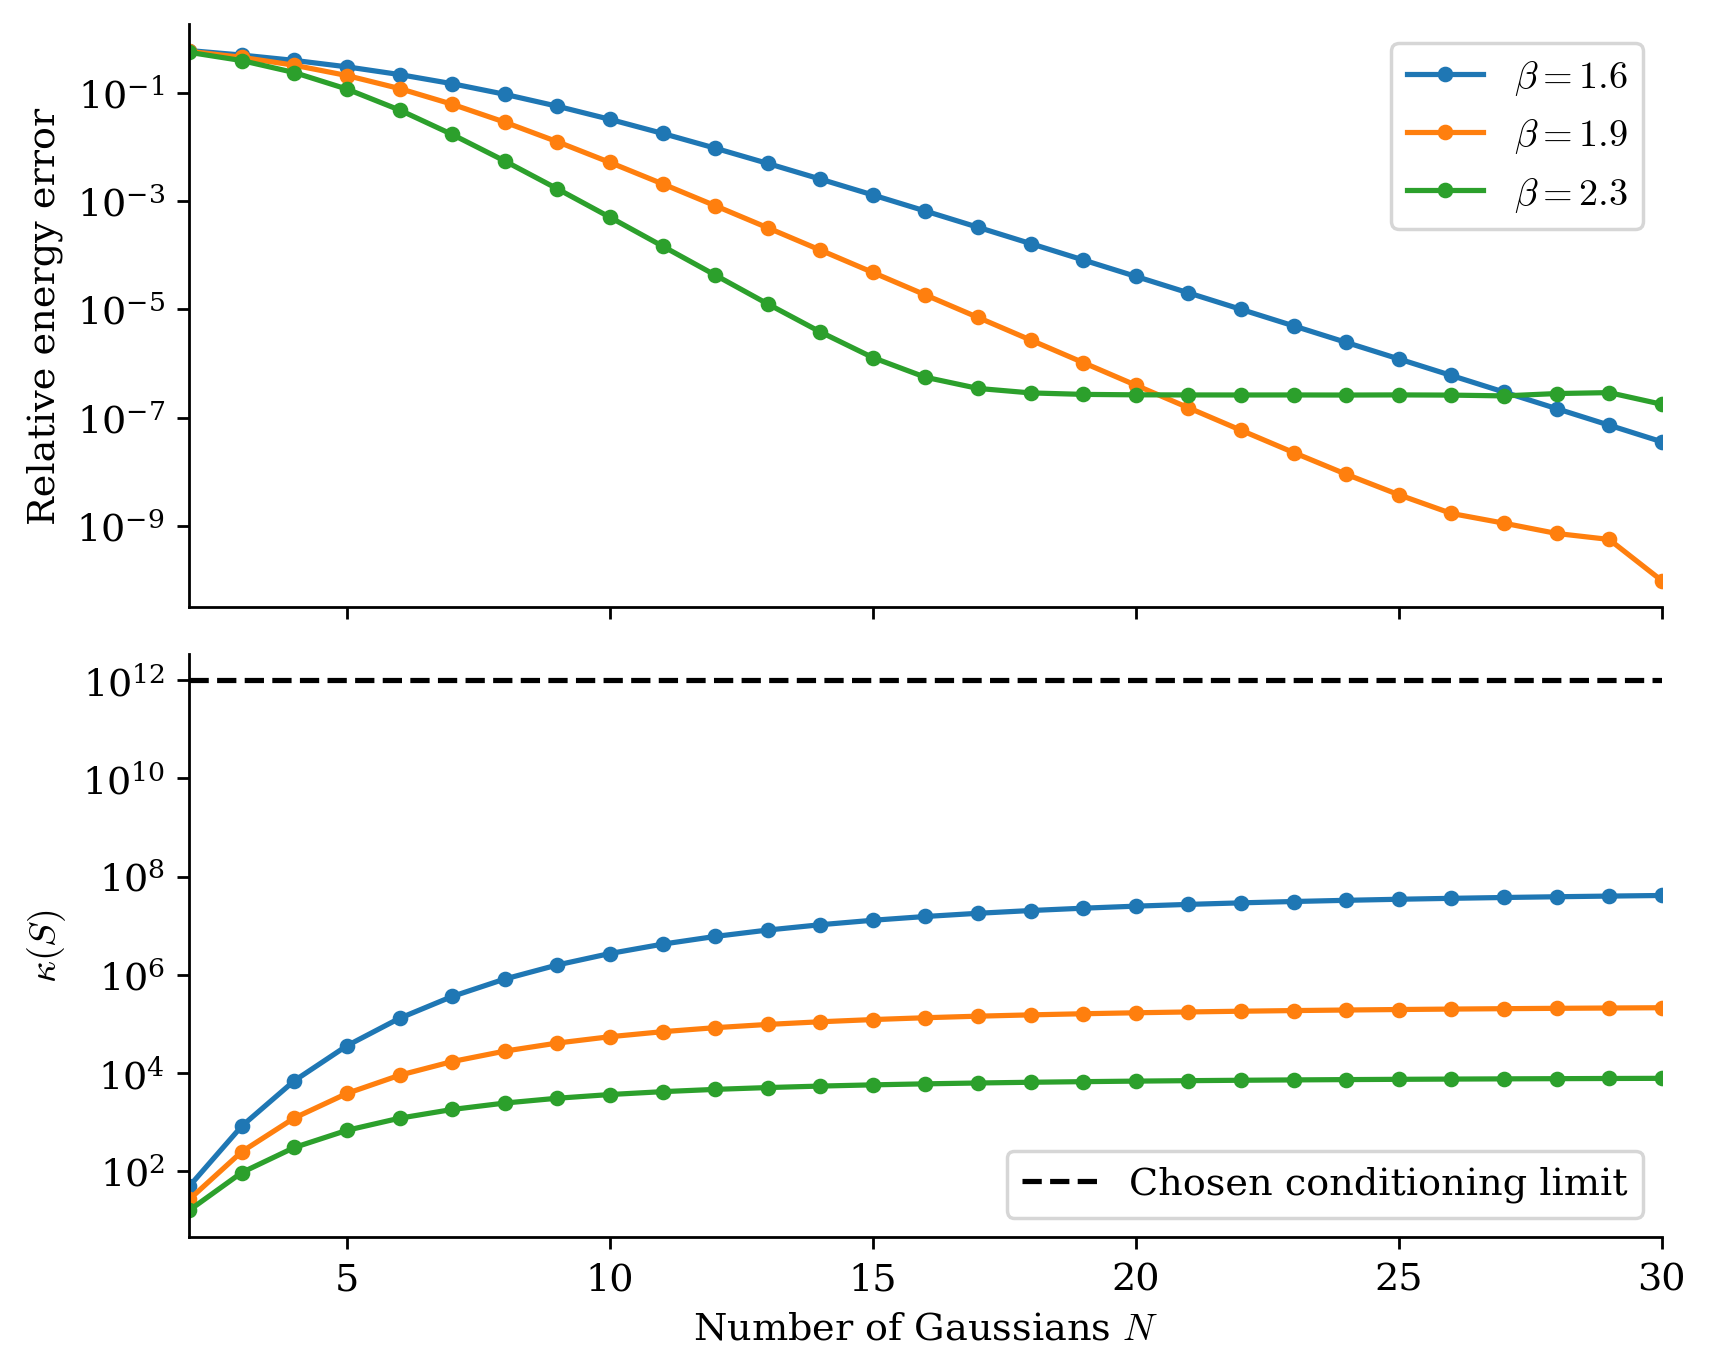
\includegraphics[width=0.80\linewidth]
{Figures/03_convergence_and_conditioning.png}
\caption{Relative hydrogen energy error and
overlap-matrix condition number against basis
size for three exponent ratios. The dashed
condition-number threshold is the screening
criterion used in the separate basis-selection
search, rather than a universal stability limit.}
\label{fig:convergence_conditioning}
\end{figure}

Figure~\ref{fig:convergence_conditioning} shows that the rate of energy convergence depends strongly
on the spacing between Gaussian exponents. With $\alpha=0.01\ \mathrm{bohr}^{-2}$ held fixed, the
three values of $\beta$ produce different convergence behaviour as $N$ increases. For the tested range, $\beta=2.3$ initially reduces the energy error more rapidly than the smaller exponent ratios. However, its improvement subsequently slows and the curve approaches a plateau. The
$\beta=1.9$ sequence continues improving over a wider range of basis sizes. This difference is important because it shows that the most effective exponent distribution depends
on the number of functions available. A ratio that gives rapid improvement for a small basis does
not necessarily provide the best approximation as the basis becomes larger.

The condition-number results provide a separate view of numerical behaviour. The overlap condition
number generally increases with basis size, particularly when successive exponents are closely
spaced. This is expected because Gaussians with similar widths overlap strongly, making some
combinations of functions difficult to distinguish numerically. However, the energy plateau for $\beta=2.3$ occurs well below the chosen condition-number threshold.
The available evidence therefore does not establish numerical instability as the cause of the
plateau.

A possible explanation follows from the structure of the even-tempered sequence. At fixed $\alpha$
and $\beta$, increasing $N$ introduces progressively narrower Gaussians without adding more diffuse
functions. Once the short-range behaviour is adequately represented, further functions may provide
little improvement if the remaining error lies in radial regions that are not well covered.
This interpretation is consistent with the sensitivity to exponent selection examined below.
However, the convergence curves alone do not isolate the source of the remaining error, so the
plateau cannot be assigned a unique cause.

\begin{figure}[htbp]
\centering
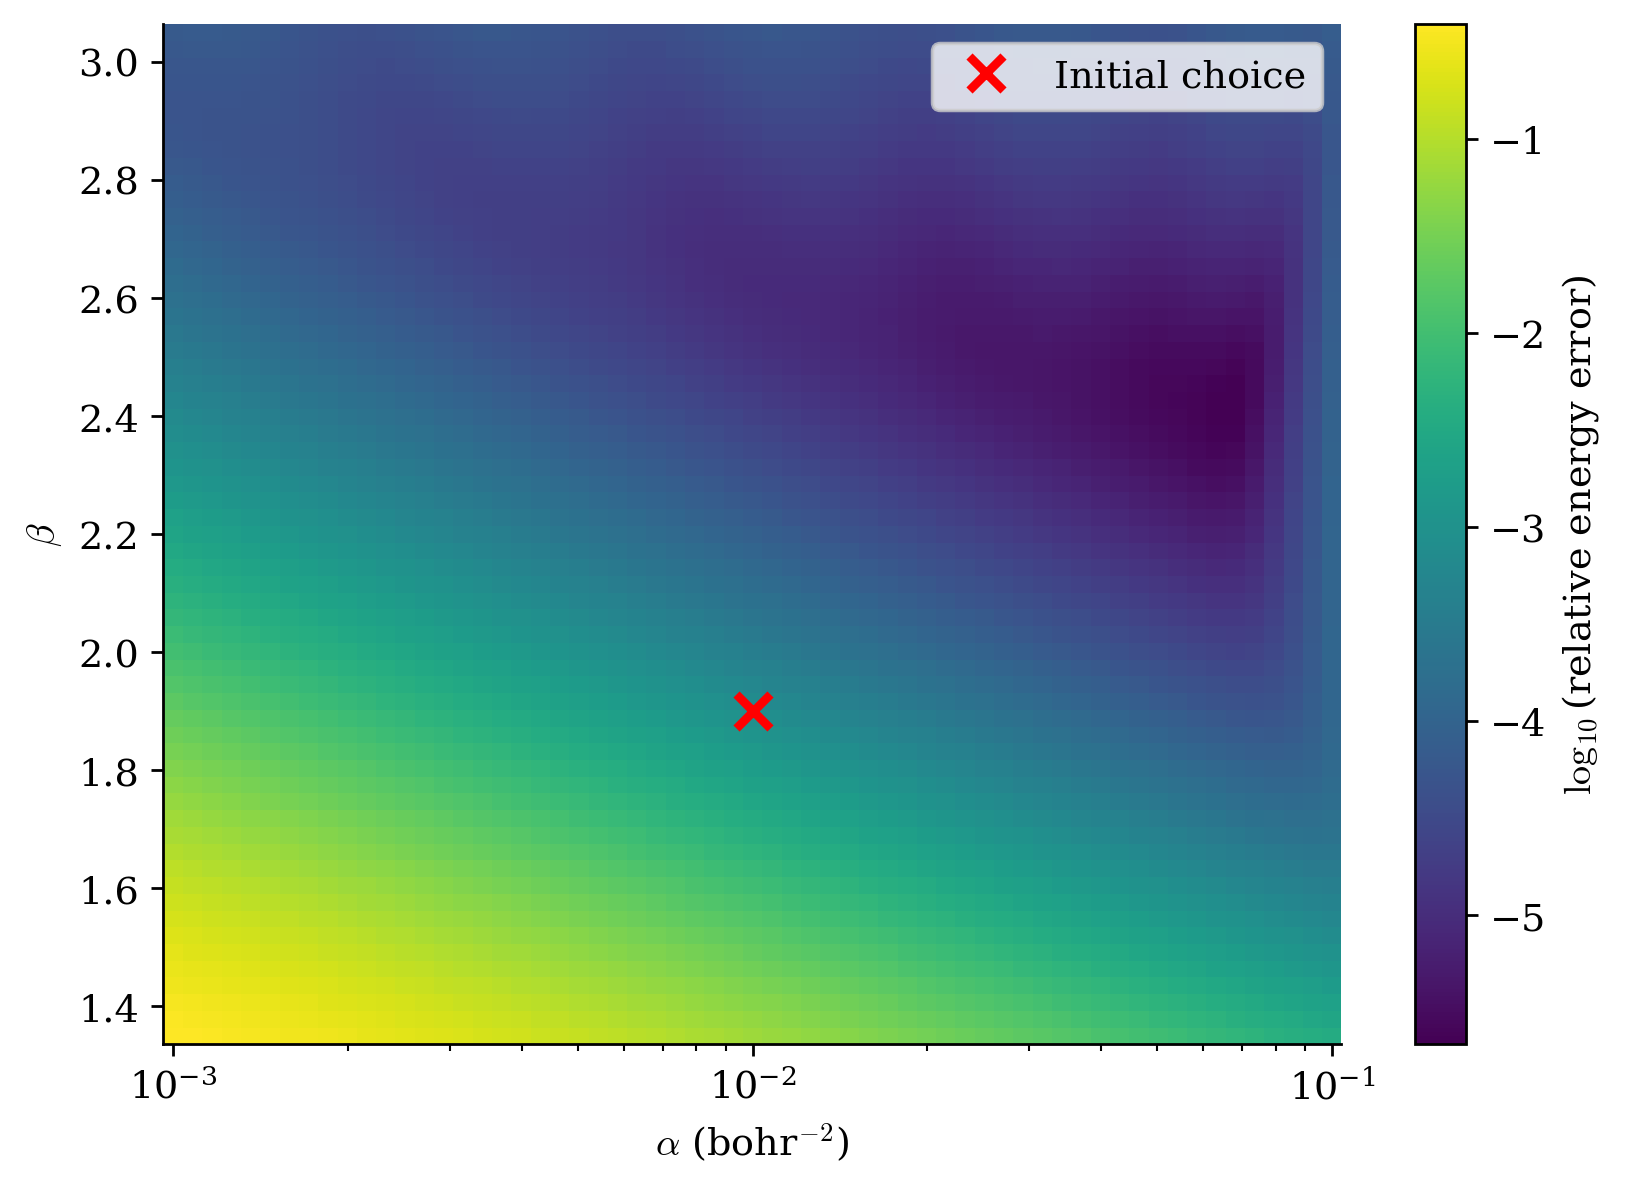
\includegraphics[width=0.80\linewidth]
{Figures/04_alpha_beta_heatmap.png}
\caption{Relative hydrogen energy error across
the tested even-tempered exponent parameters
at $N=12$. The red cross marks the reference
parameters $\alpha=0.01\ \mathrm{bohr}^{-2}$
and $\beta=1.9$, not an optimised solution.}
\label{fig:parameter_map}
\end{figure}

Figure~\ref{fig:parameter_map} examines the combined effect of $\alpha$ and $\beta$ at fixed basis
size. The variation in energy error shows that the reference parameters are not uniquely favourable
and that the distribution of exponents has a substantial influence on the quality of the
approximation. The smallest exponent $\alpha$ determines the broadest Gaussian, while $\beta$ determines how
rapidly the sequence reaches narrower functions. Their effects are connected because the largest
exponent is $\lambda_N=\alpha\beta^{N-1}$.
Changing $\alpha$ shifts the overall exponent range, whereas changing $\beta$ alters both the
spacing and the extent of that range. Consequently, the parameters cannot be assessed independently
when judging the radial coverage of a finite basis.
The parameter map therefore provides a physical explanation for the different convergence curves. Adding functions is useful only when their widths improve the representation of the wavefunction. A smaller basis with appropriately chosen exponents can outperform a larger basis whose exponent
distribution is less suitable.

To quantify this effect, a discrete parameter search was used to identify the smallest tested basis
satisfying selected relative energy-error targets. The results are given in Table~\ref{tab:basis_selection}.

\begin{table}[H]
\centering
\caption{Smallest tested Gaussian bases satisfying
selected relative energy-error targets. Results
are restricted to the discrete parameter grid
described in Chapter~\ref{chap:methodology},
with $\kappa(\mathbf S)\leq10^{12}$.}
\label{tab:basis_selection}
\begin{tabular}{ccccc}
\hline
Target error & $N$ &
$\alpha\ (\mathrm{bohr}^{-2})$ &
$\beta$ & Actual error\\
\hline
$10^{-2}$ & 5 & $0.100000$ & $2.8$
    & $2.5755\times10^{-3}$\\
$10^{-3}$ & 6 & $0.100000$ & $2.8$
    & $6.2944\times10^{-4}$\\
$10^{-4}$ & 8 & $0.068129$ & $2.8$
    & $6.6406\times10^{-5}$\\
\hline
\end{tabular}
\end{table}

The search evaluated 1,365 parameter combinations before its early-stopping condition was reached.
All attempted generalised eigenvalue solves completed successfully. For the least restrictive target, a relative energy error below $10^{-2}$ was achieved with five
Gaussians. Six functions were sufficient for an error below $10^{-3}$, while the strictest target of
$10^{-4}$ was reached with eight functions.

The eight-function basis uses $\alpha=0.068129\ \mathrm{bohr}^{-2}$ and $\beta=2.8$, giving a
relative energy error of $6.6406\times10^{-5}$.
This is a substantial improvement over the twelve-function reference basis, whose relative energy
error is $8.2170\times10^{-4}$. The selected basis achieves an error approximately 12.4 times smaller using four fewer functions. The result demonstrates that increasing basis size is not necessarily the most efficient way to
improve accuracy. Selecting exponents that better represent the relevant radial length scales can be
more effective than adding functions to a fixed sequence.

An important qualification is that all three selected values of $\beta$ lie at the upper boundary of
the tested search range, $\beta=2.8$. Two of the selected $\alpha$ values also lie at their upper
boundary. These boundary selections suggest that the chosen parameter ranges may influence the reported
results. Extending the search beyond these limits or using a finer grid could identify other
successful combinations, potentially with fewer functions.
The results therefore establish the smallest successful basis sizes within the tested discrete grid,
not globally optimal Gaussian bases. Nevertheless, the comparison with the reference calculation
provides clear evidence that exponent selection is central to variational accuracy.


% 4.3 WAVEFUNCTION ACCURACY AND NEAR-NUCLEAR BEHAVIOUR



\section{Wavefunction Accuracy and Near-Nuclear Behaviour}

\begin{figure}[htbp]
\centering
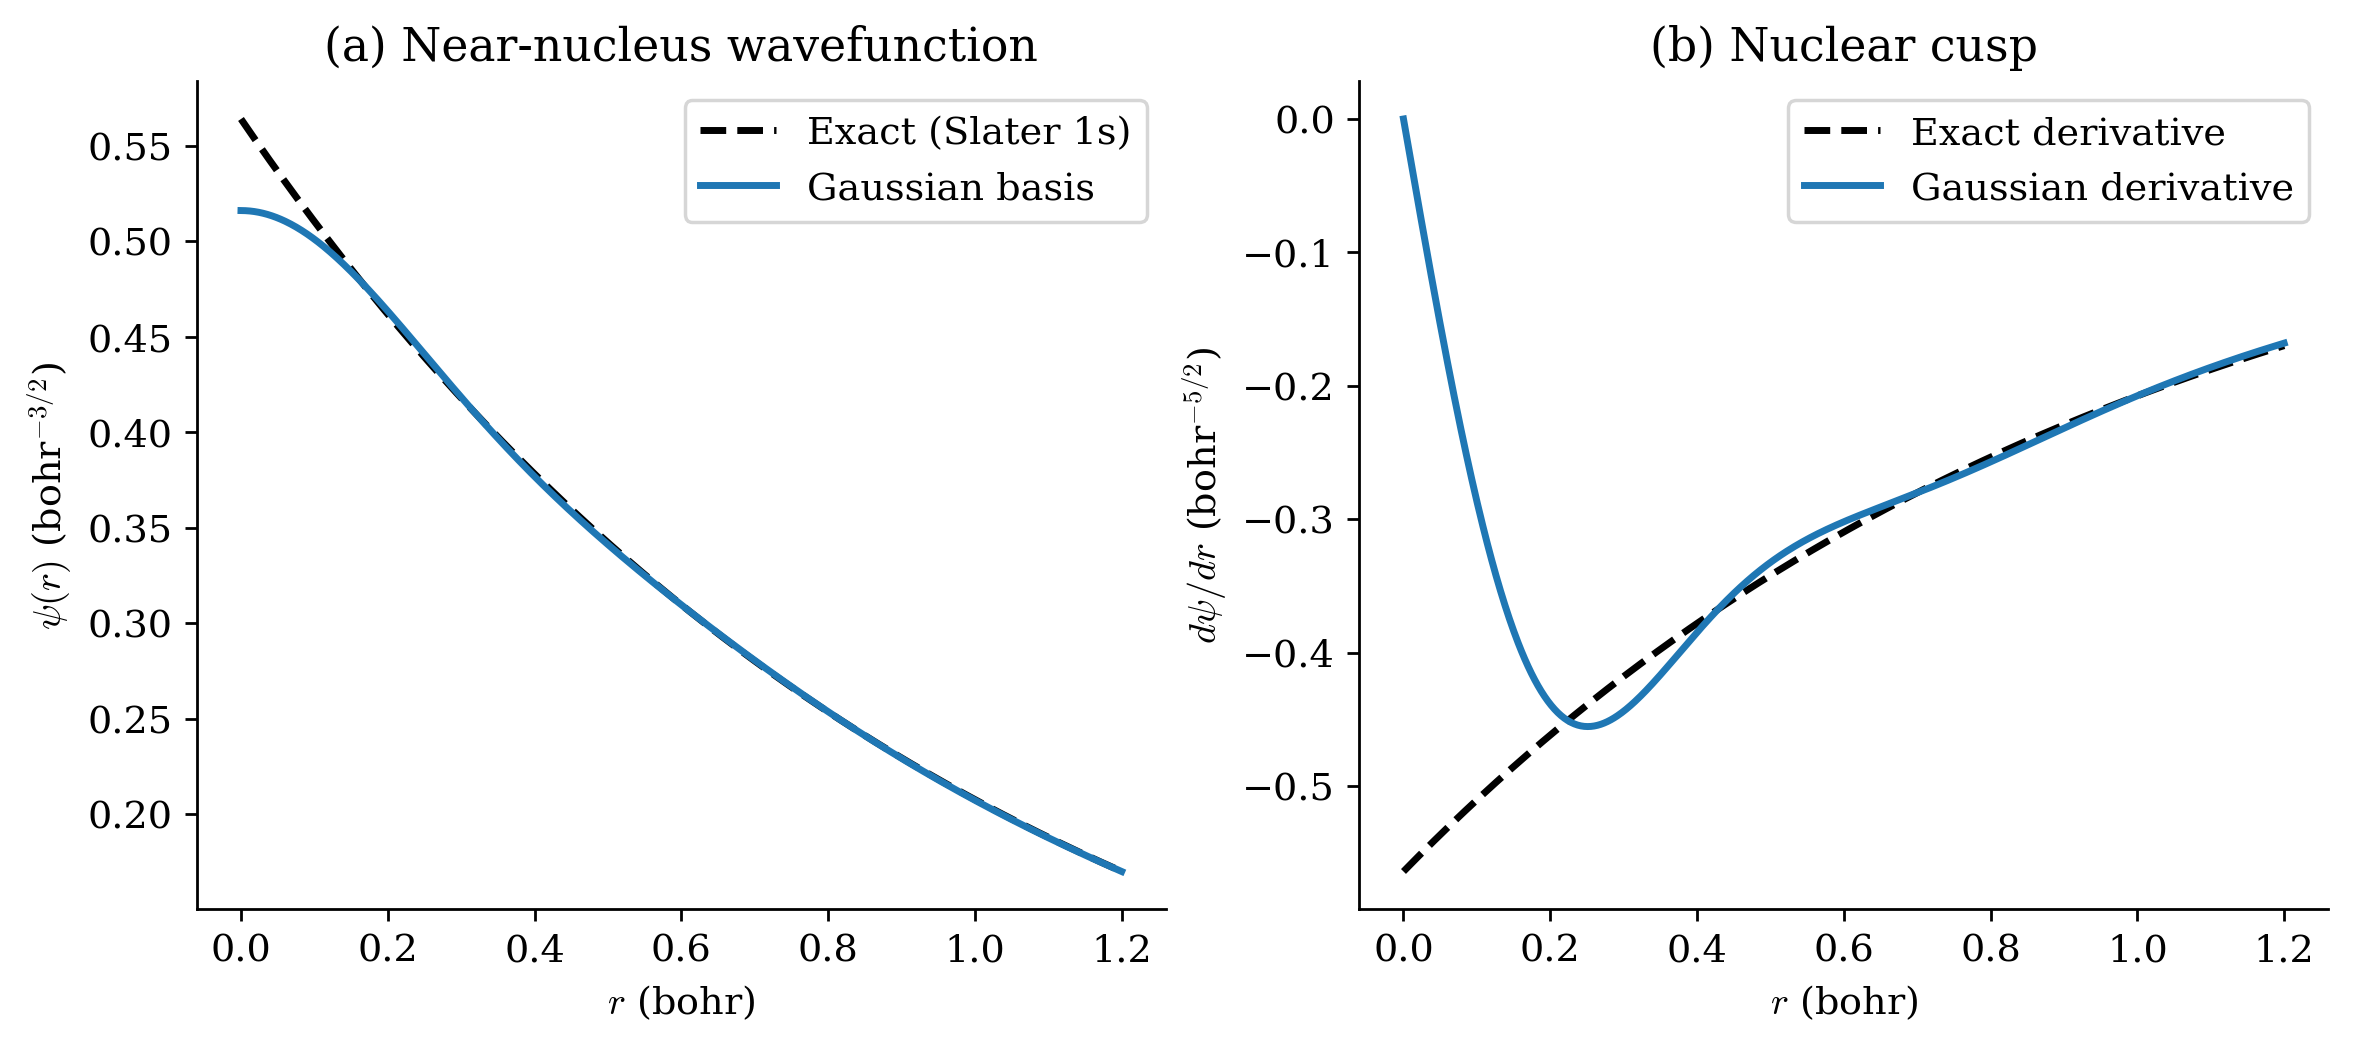
\includegraphics[width=0.9\linewidth]
{Figures/08_nuclear_cusp.png}
\caption{Exact and Gaussian hydrogen wavefunctions
and radial derivatives near the nucleus. The
Gaussian derivative vanishes at the origin,
whereas the exact derivative satisfies the
electron--nucleus cusp condition.}
\label{fig:nuclear_cusp}
\end{figure}

Figure~\ref{fig:nuclear_cusp} examines the near-nuclear region more closely, where the reference
wavefunction shows its largest visible discrepancy.
For hydrogen, the exact radial
derivative at the origin is
\[
    \psi_{1s}'(0)
    =-\frac{1}{\sqrt{\pi}}\
      \mathrm{bohr}^{-5/2}.
\]
By contrast, the derivative
of the finite Gaussian
expansion is zero.

This difference follows from the functional form of the basis rather than the numerical solution.
Every centred spherical Gaussian has zero radial derivative at the origin, so any finite linear
combination also has zero derivative there.
The exact hydrogenic wavefunction instead satisfies the non-zero electron--nucleus cusp condition in
Eq.~\eqref{eq:cusp_condition} \cite{Kato,Kutzelnigg1994}.
Increasing the number of Gaussians or changing their coefficients can improve the approximation over
a small but finite region near the nucleus. However, no finite combination of these functions can
reproduce the exact derivative at $r=0$.
This is an inherent limitation of the finite spherical Gaussian basis and cannot be removed simply
by solving the variational problem more accurately.

\begin{figure}[htbp]
\centering
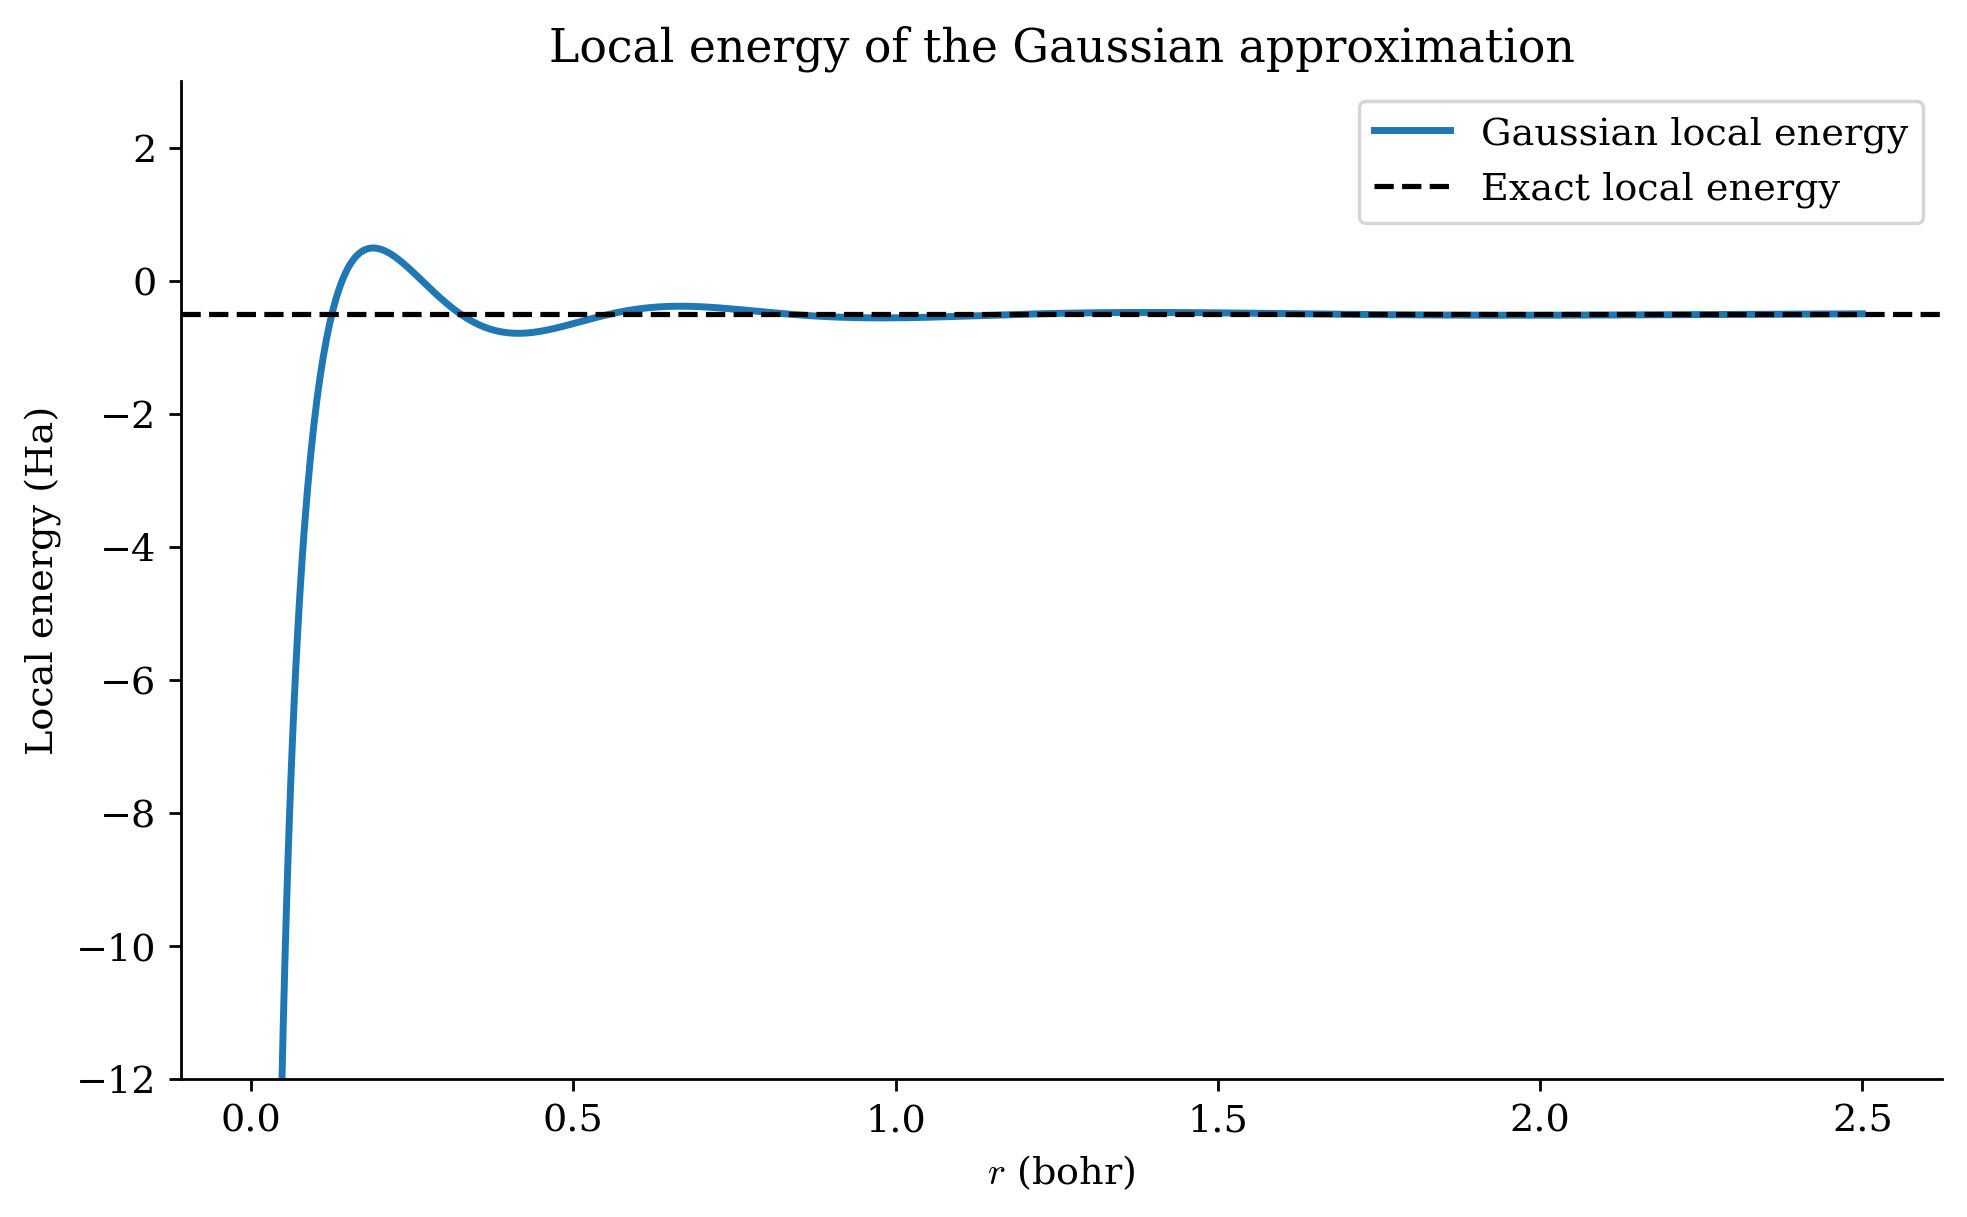
\includegraphics[width=0.82\linewidth]
{Figures/09_local_energy.png}
\caption{Local energy of the Gaussian hydrogen
approximation compared with the constant exact
ground-state energy. The strong near-nuclear
variation results from the missing cusp.}
\label{fig:local_energy}
\end{figure}

The local-energy comparison in Fig.~\ref{fig:local_energy} shows a further consequence of the
missing cusp. For an exact eigenstate, the local energy defined in Eq.~\eqref{eq:local_energy} equals the
corresponding eigenvalue wherever the wavefunction is non-zero. For hydrogen, this is the constant
value $-0.5$ Hartree.

The Gaussian approximation behaves differently. For a finite spherical Gaussian expansion, the
kinetic-energy contribution remains finite as $r\to0$, whereas the Coulomb potential contains the
singular term $-Z/r$. Because the approximate wavefunction is non-zero at the nucleus, its local energy diverges negatively as $r\to0^+$. The difference is directly related to the cusp condition. In the exact state, the non-zero radial derivative produces a singular kinetic contribution that cancels the Coulomb singularity. The finite
Gaussian expansion cannot provide the same cancellation.

Importantly, this local divergence does not make the total variational energy infinite. The energy
expectation value is integrated over three-dimensional space, with radial volume element $4\pi
r^2\,\mathrm dr$. Near the nucleus, the Coulomb contribution therefore behaves as an integrable term proportional to $r\,\mathrm dr$ for a finite, non-zero wavefunction amplitude. The total energy remains finite even though the local energy diverges. This explains how a Gaussian
basis can give an accurate integrated energy while retaining a systematic error in its behaviour at
the nucleus.

\begin{figure}[htbp]
\centering
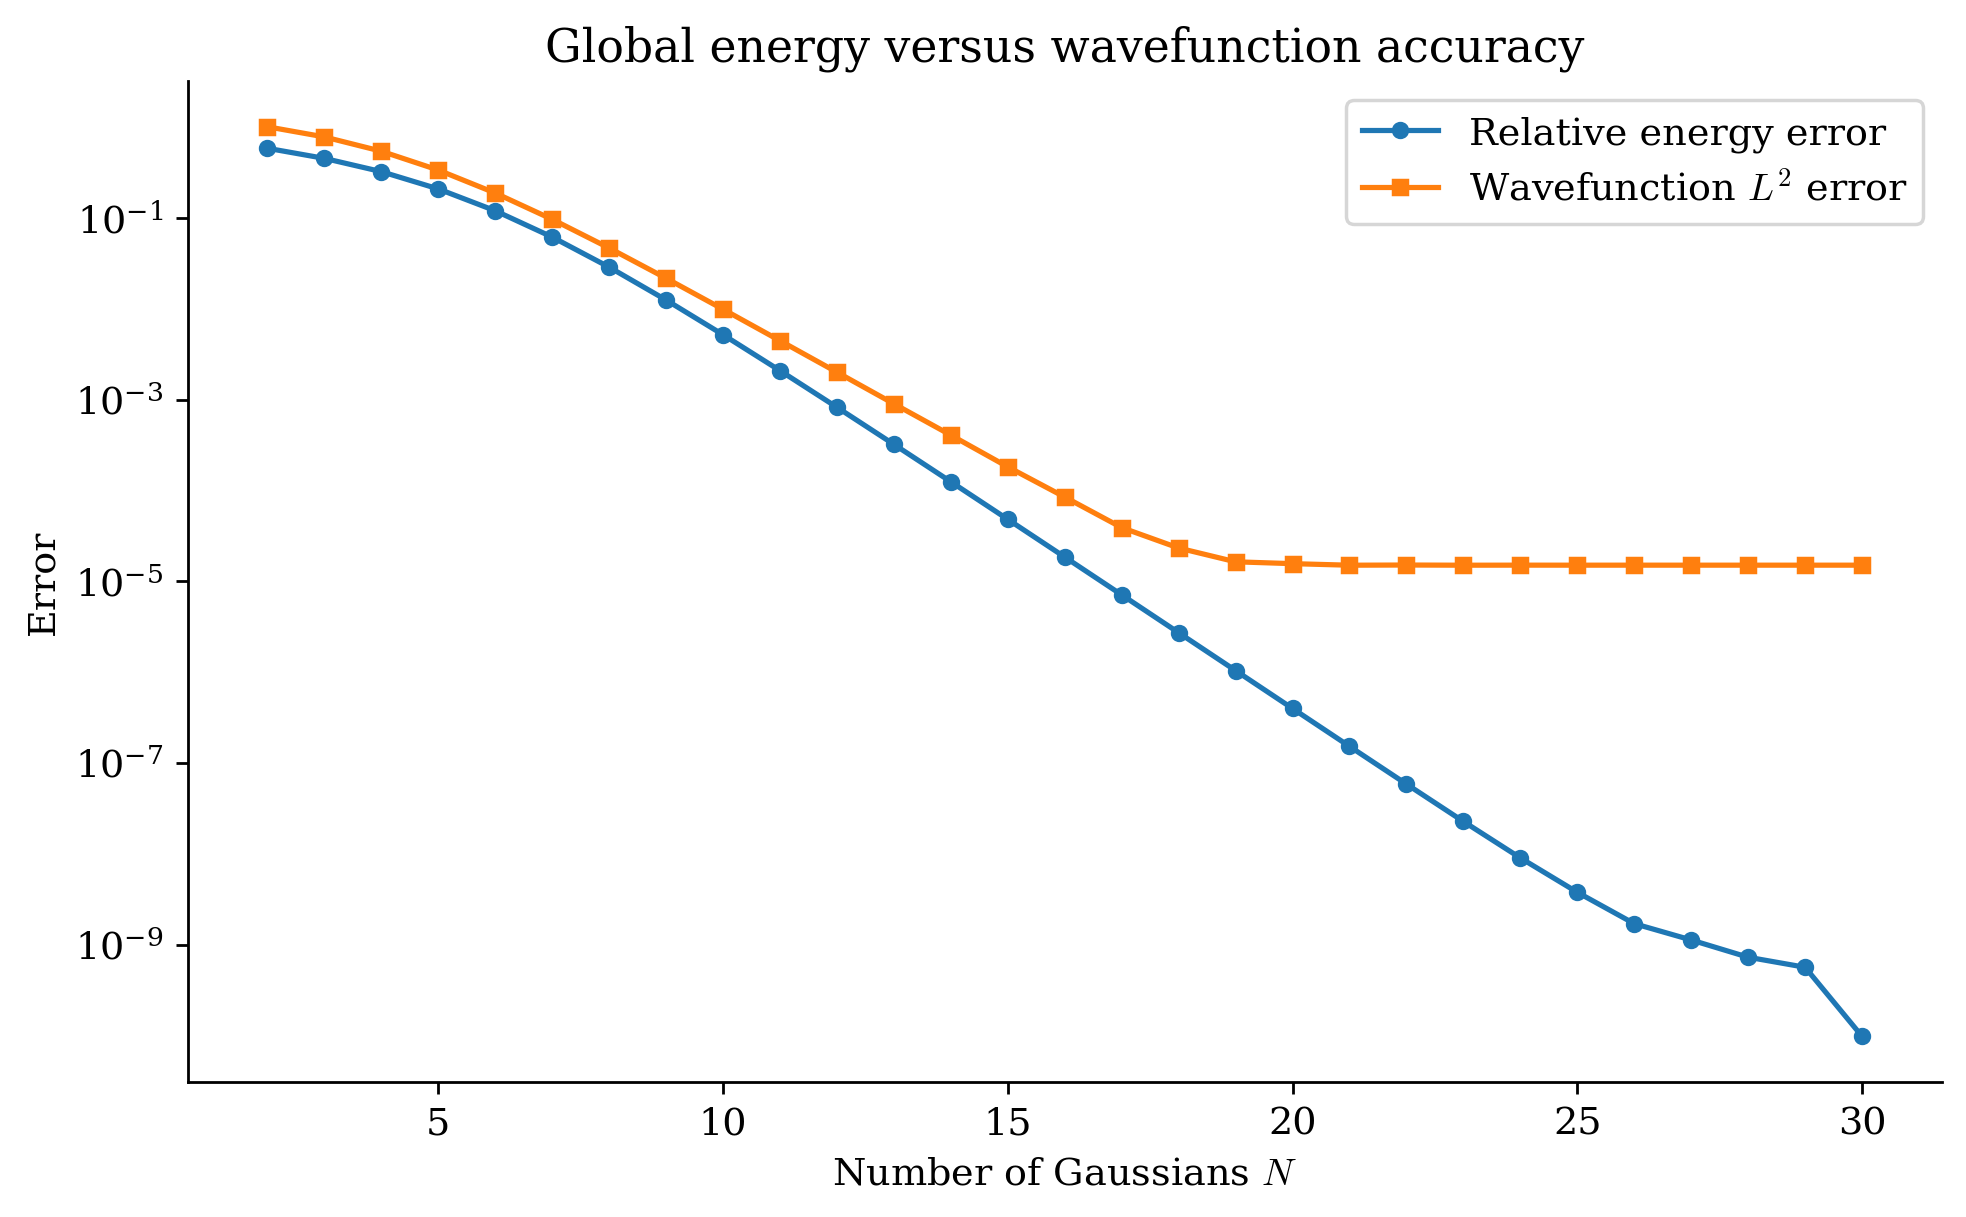
\includegraphics[width=0.85\linewidth]
{Figures/10_energy_vs_wavefunction_error.png}
\caption{Convergence of the relative variational
energy error and the three-dimensional $L^2$
wavefunction error with increasing Gaussian
basis size. The two quantities converge at
different rates.}
\label{fig:energy_wavefunction_convergence}
\end{figure}

Figure~\ref{fig:energy_wavefunction_convergence} compares the relative energy error with the
three-dimensional $L^2$ wavefunction error as the basis size increases. Both quantities generally decrease with increasing $N$, but their rates of convergence are
different. The energy becomes highly accurate before the wavefunction error has decreased by a
comparable amount. For a normalised approximate ground state, Eq.~\eqref{eq:variational_error} expresses the variational energy error as a quadratic, energy-weighted function of the wavefunction error, whereas the $L^2$ norm measures the wavefunction difference directly. The energy can therefore improve substantially even when a small spatial error remains. This explains why energy convergence alone is insufficient to establish the
accuracy of the reconstructed wavefunction, although it does not identify the cause of the
$L^2$-error plateau discussed below.

The wavefunction $L^2$ error begins to plateau at approximately $N=20$, remaining near $1.5\times10^{-5}$ despite continued improvement in the variational energy.
At $N=30$, the calculated wavefunction error is
\[
    \varepsilon_\psi
    \approx
    1.50493050\times10^{-5}.
\]
Adaptive numerical integration and fine-grid integration agree to a relative difference of $2.127\times10^{-10}$.
The close agreement indicates that the observed wavefunction error is not simply an inconsistency
between the two integration methods. It also supports the reliability of the numerical evaluation of
the $L^2$ norm.

However, the calculations do not establish the cause of the apparent wavefunction-error plateau. Possible influences include the distribution of Gaussian exponents, the remaining limitations of the finite basis and numerical sensitivity at larger $N$. The present results do not distinguish between these possibilities.
The plateau should therefore not be interpreted as a fundamental accuracy limit of Gaussian basis
expansions. Further calculations with different exponent ranges, larger bases or higher numerical
precision would be needed to identify its origin.

\begin{figure}[htbp]
\centering
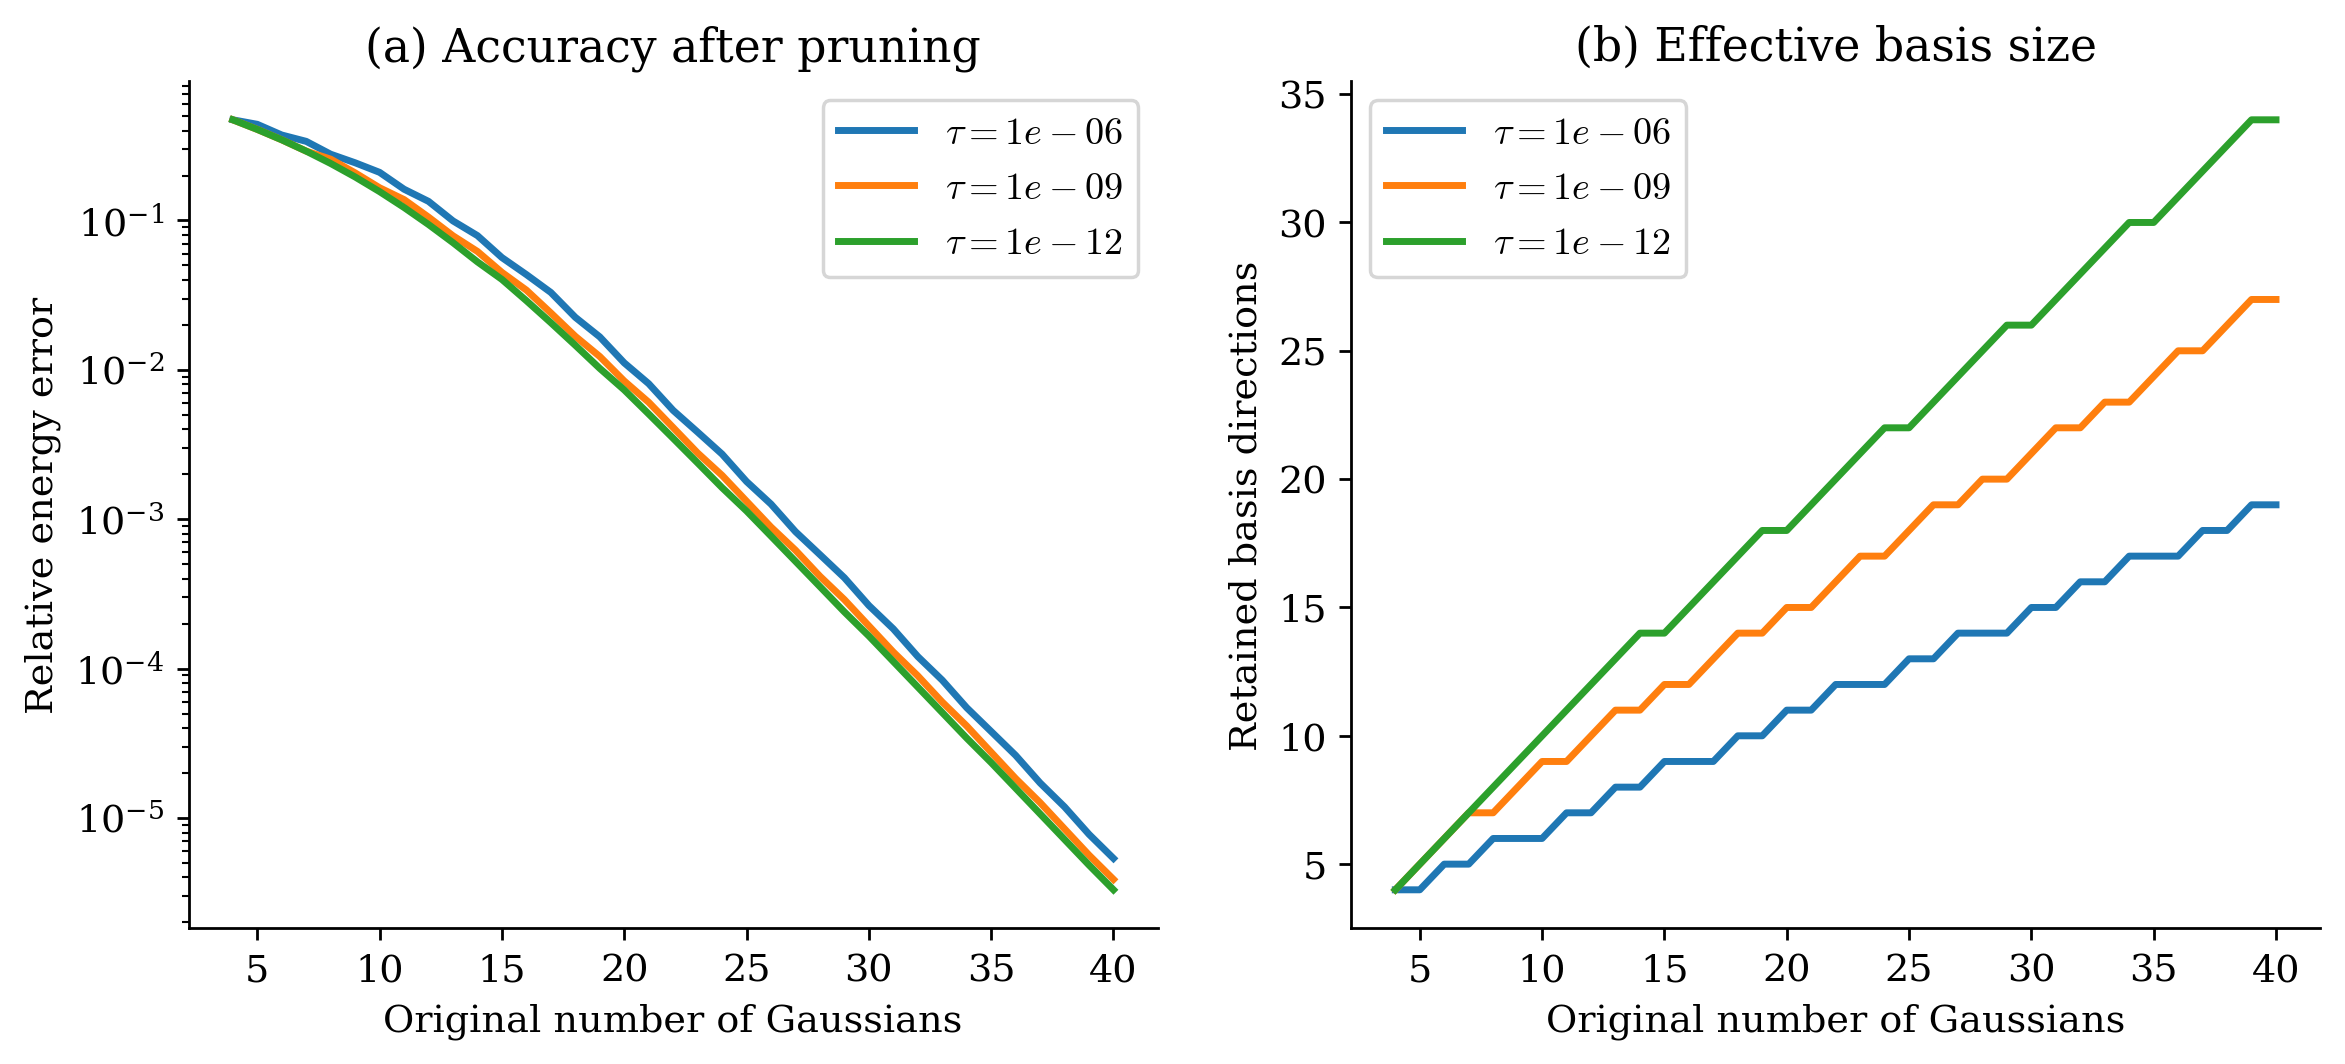
\includegraphics[width=1\linewidth]
{Figures/11_basis_pruning.png}
\caption{Canonical orthogonalisation test showing (a) relative ground-state energy error and (b) retained basis dimension for three overlap-eigenvalue thresholds. Following re-orthogonalisation, all tested basis sizes passed the numerical reliability checks, giving continuous energy-error curves.}
\label{fig:basis_pruning}
\end{figure}

The canonical orthogonalisation results in Fig.~\ref{fig:basis_pruning} examine the effect of removing nearly dependent combinations of Gaussian functions. As the exponent ratio approaches unity, neighbouring Gaussians become increasingly similar, producing small eigenvalues of the overlap matrix. Pruning these directions reduces the effective dimension of the variational space, but can also remove combinations that contribute to the accuracy of the ground state.

All 111 pruning calculations passed the implemented reliability checks following re-orthogonalisation, with no exclusions at any of the three thresholds. The energy-error curves consequently extend across the complete tested range, $N=4,\ldots,40$. No energy-error values are omitted from the final plot.
At $N=40$, the thresholds $10^{-6}$, $10^{-9}$ and $10^{-12}$ retain 19, 27 and 34 basis directions, respectively. The most aggressive threshold therefore removes 21 of the original 40 directions, a reduction of $52.5\%$. The intermediate and least aggressive thresholds remove $32.5\%$ and $15.0\%$, respectively. These reductions show how strongly the closely spaced Gaussians overlap: many nominal basis functions add little independent variational freedom. The energy-error curves reveal the corresponding trade-off within this experiment, with smaller thresholds generally giving lower errors and larger thresholds producing more compact bases.

The results demonstrate that nominal basis size can substantially overstate the number of distinct directions needed for a given level of energy accuracy. Canonical orthogonalisation offers a practical way to control near-linear dependence, provided that the retained dimension, variational error and numerical checks are assessed together. Passing those checks establishes the reliability of the reported calculations under the chosen criteria, not a universal guarantee of stability for arbitrary basis parameters.



% 4.4 TRANSFERABILITY AND NUCLEAR-CHARGE SCALING


\section{Transferability and Nuclear-Charge Scaling}

The final calculations examine whether a Gaussian basis constructed for hydrogen can be reused for
more strongly bound one-electron ions.
The exact hydrogenic ground state contracts on a characteristic length scale proportional to $1/Z$.
Consequently, an unchanged hydrogen exponent sequence becomes increasingly broad relative to the
physical electron distribution as the nuclear charge increases.

\begin{figure}[htbp]
\centering
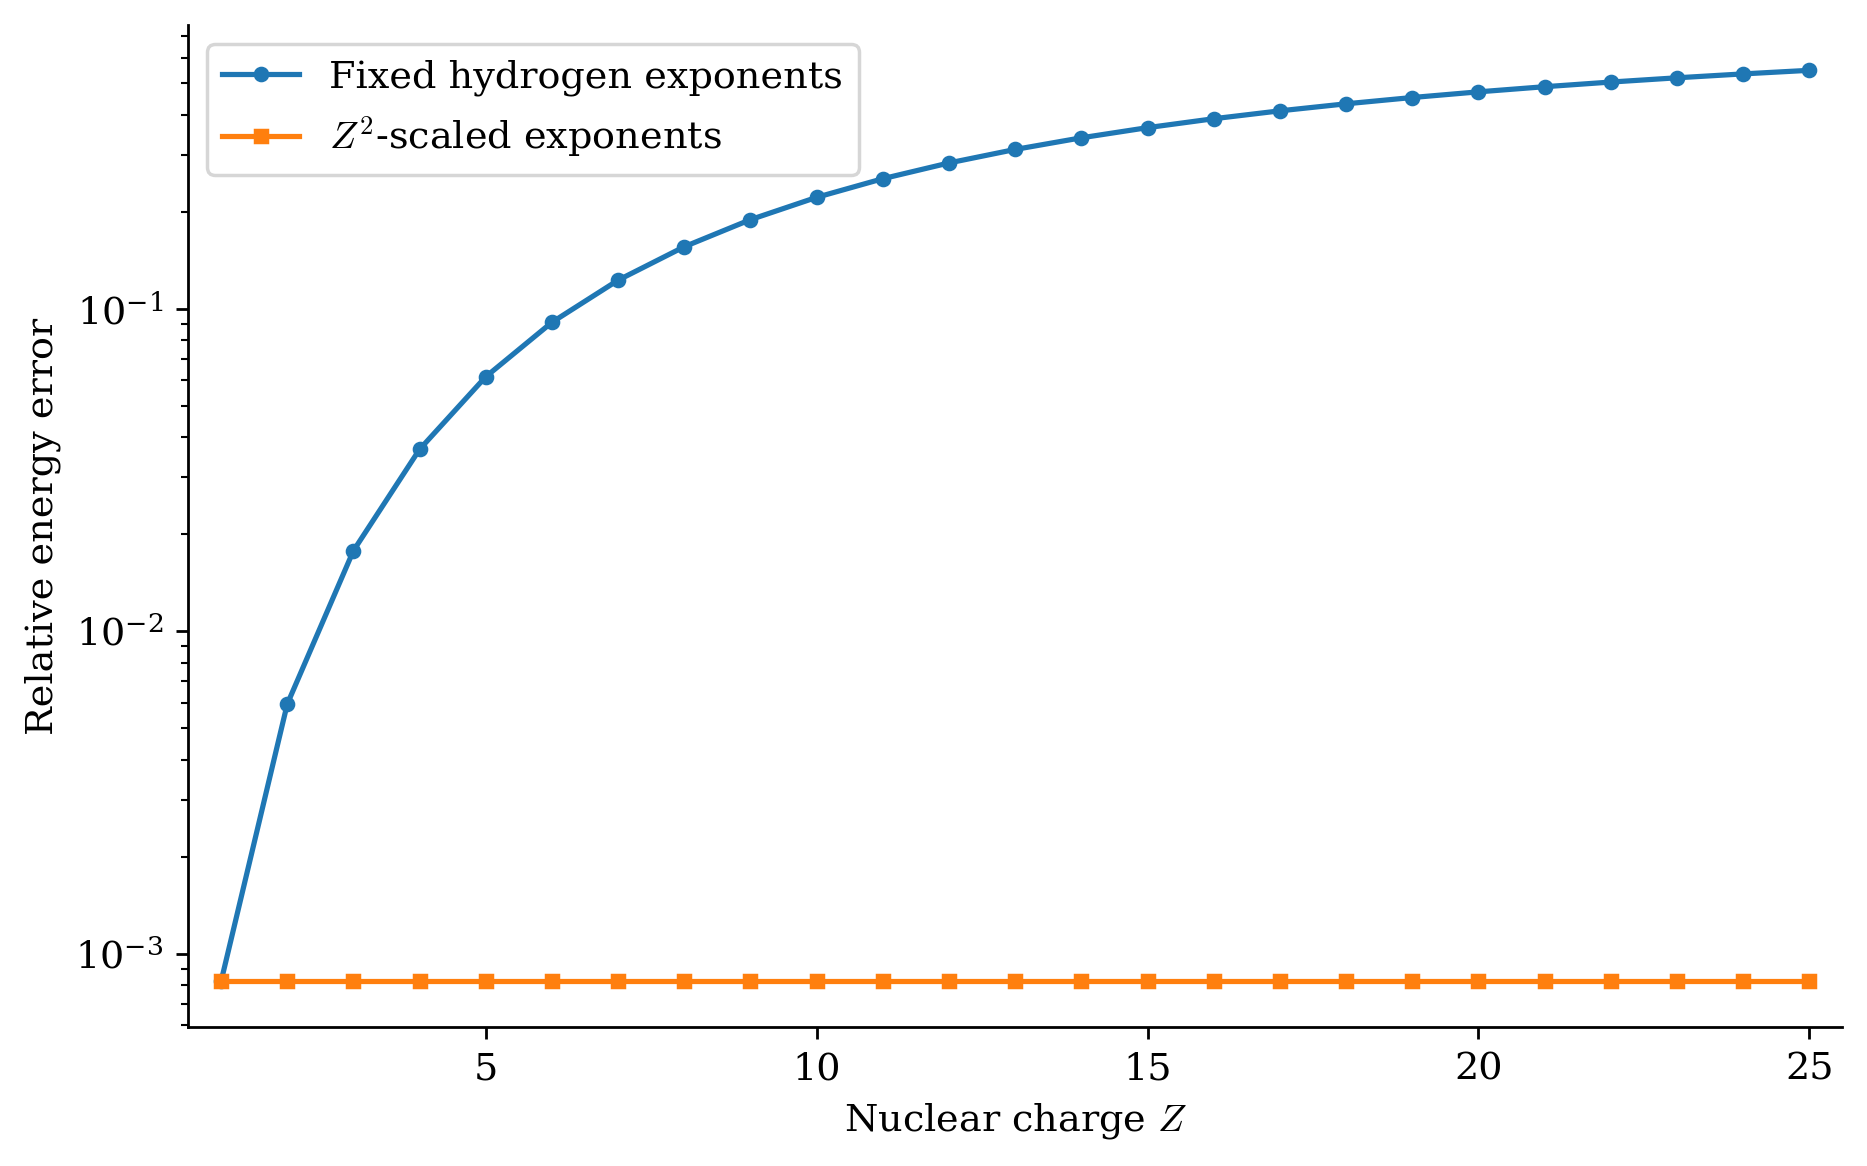
\includegraphics[width=0.82\linewidth]
{Figures/05_fixed_vs_scaled_charge.png}
\caption{Relative ground-state energy error
against nuclear charge for fixed hydrogen
exponents and exponents scaled by $Z^2$.
The scaled basis preserves the hydrogen
relative energy error.}
\label{fig:charge_transfer}
\end{figure}

Figure~\ref{fig:charge_transfer} compares the relative energy errors obtained with fixed and
$Z^2$-scaled exponents. For the unchanged hydrogen basis, the relative error increases from $8.2170\times10^{-4}$ at $Z=1$ to approximately $0.549$ at $Z=25$.
The fixed basis therefore becomes progressively less effective at representing the more strongly
bound ground states. By contrast, the $Z^2$-scaled basis retains the hydrogen relative energy error throughout the tested range.
This agrees with
Eq.~\eqref{eq:scaled_energy},
which predicts:
\[
    E_{\mathrm G}(Z)
    =Z^2E_{\mathrm G}(1),
\]
when the Gaussian exponents are scaled consistently.
Since the exact hydrogenic energy also scales as $Z^2$, the relative energy error remains unchanged.

Although the scaled basis maintains a constant
relative energy error, this result applies within
the non-relativistic hydrogenic model. As $Z$
increases, the characteristic electron velocity
scales approximately as $v/c\sim Z\alpha_{\mathrm{fs}}$,
where $\alpha_{\mathrm{fs}}\approx1/137$ is the
fine-structure constant. Relativistic corrections
therefore become increasingly important at higher
nuclear charges and are not included in the
present calculations.


\begin{table}[htbp]
\centering
\caption{Exact and variational ground-state energies for
hydrogen and hydrogenic manganese ($\mathrm{Mn}^{24+}$).
Exact values follow from $E_{1s}=-Z^2/2$ (Section~2.1);
the fixed- and scaled-exponent results are calculated
as described in Section~3.2. Energies are in Hartree.}
\label{tab:charge_energies}
\begin{tabular}{lccc}
\hline
System & Exact & Fixed exponents & Scaled exponents \\
\hline
H ($Z=1$)
    & $-0.500000$
    & $-0.499589$
    & $-0.499589$ \\
$\mathrm{Mn}^{24+}$ ($Z=25$)
    & $-312.500000$
    & $-140.956593$
    & $-312.243220$ \\
\hline
\end{tabular}
\end{table}

The $Z=25$ energies in Table~\ref{tab:charge_energies} show the magnitude of the difference.
For hydrogenic $\mathrm{Mn}^{24+}$, the exact ground-state energy is $-312.5$ Hartree. Using the unchanged hydrogen basis gives $-140.95659344$ Hartree, corresponding to a relative energy error of approximately $54.9\%$.
With $Z^2$-scaled exponents, the calculated energy becomes $-312.24322013$ Hartree, reducing the
relative error to approximately $0.0822\%$. Compared with the fixed basis, this is a reduction
in relative energy error by a factor of approximately 668, without increasing the number of
Gaussian functions. The comparison demonstrates that matching the exponent distribution to the
physical length scale can be more effective than simply enlarging a poorly matched basis.

The improvement follows directly from the coordinate transformation $\rho=Zr$. In the scaled coordinate, the Gaussian exponent appears through the combination $\lambda_i/Z^2$. Multiplying each exponent by $Z^2$ therefore preserves the original distribution of Gaussian widths relative to the contracted orbital.
The exponent scaling thus adapts the existing basis to the contracted orbital, rather than introducing additional functions.

\begin{figure}[htbp]
\centering
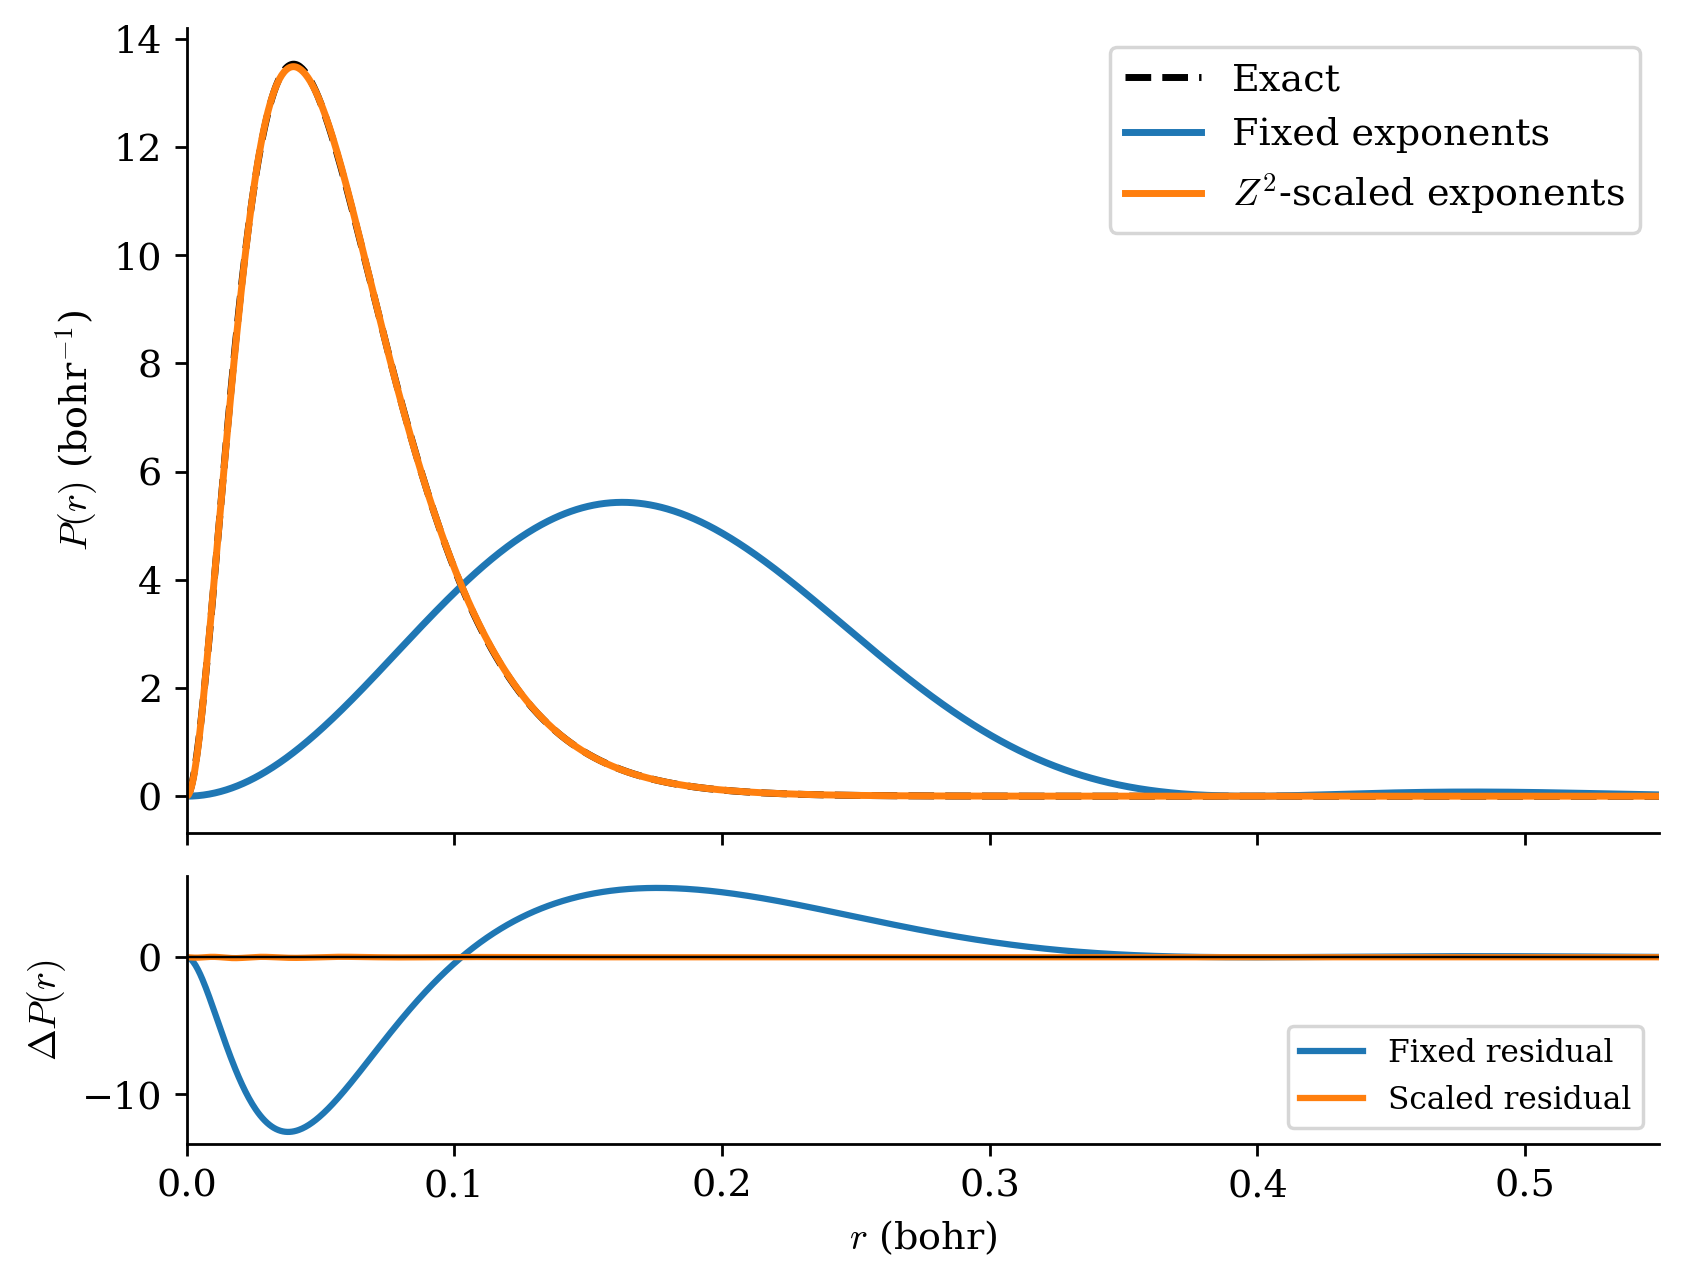
\includegraphics[width=0.9\linewidth]
{Figures/06_manganese_radial_comparison.png}
\caption{Exact, fixed-basis and
$Z^2$-scaled radial probability
distributions for hydrogenic
$\mathrm{Mn}^{24+}$, including
residuals relative to the exact
distribution.}
\label{fig:manganese_radial}
\end{figure}

The radial probability distributions in Fig.~\ref{fig:manganese_radial} show why the fixed basis
performs poorly. The exact $\mathrm{Mn}^{24+}$ ground state is strongly concentrated near the nucleus. The unchanged
hydrogen basis places too much probability at larger radii and does not reproduce the required
contraction. The scaled basis instead follows the exact radial distribution much more closely.
The improvement is therefore not confined to the variational energy. Scaling the exponents also
gives a substantially better description of the spatial electron distribution. This comparison is important because it connects the large energy error of the fixed basis to a
physically identifiable problem: its Gaussian widths are poorly matched to the size of the orbital.

\begin{figure}[htbp]
\centering
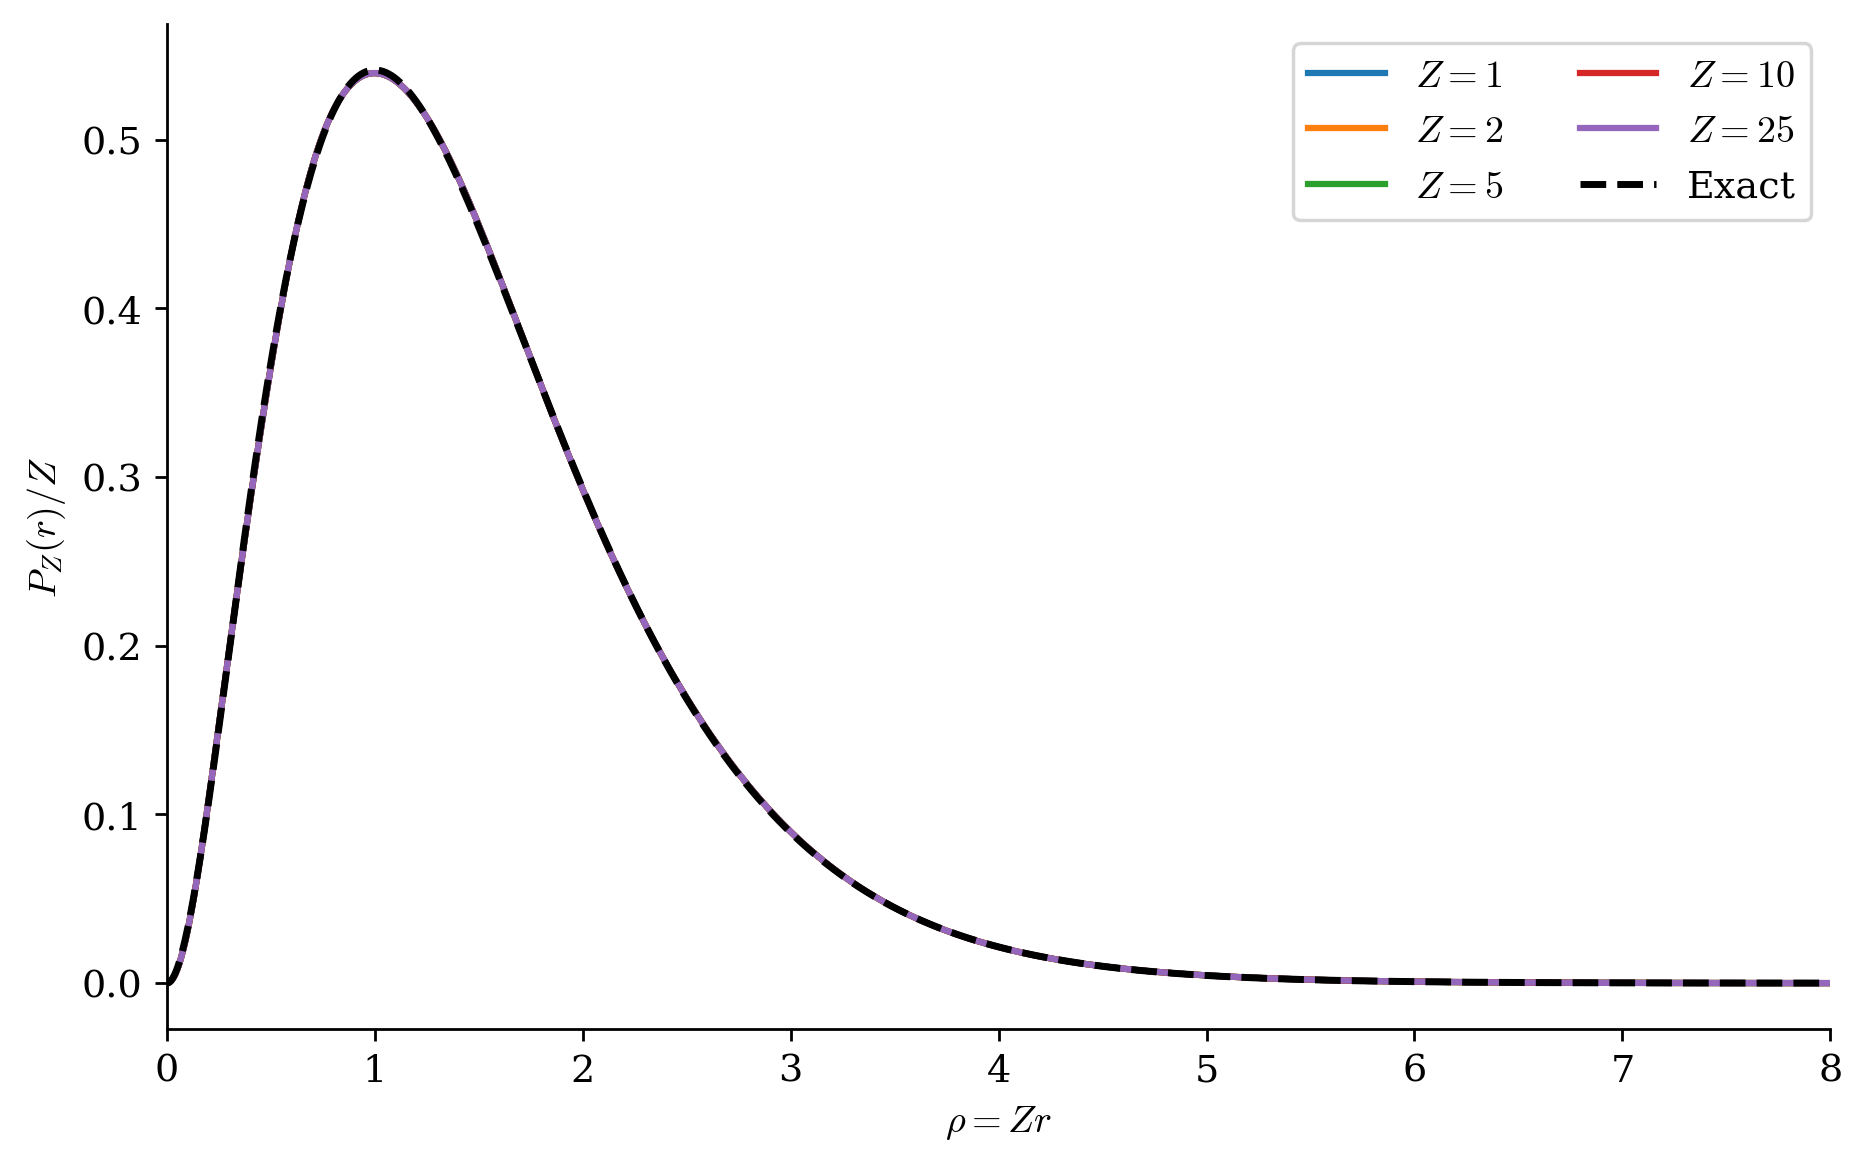
\includegraphics[width=0.82\linewidth]
{Figures/07_scaling_collapse.png}
\caption{Scaled radial probability
$P_Z(\rho/Z)/Z$ against
$\rho=Zr$ for several nuclear
charges. The overlapping curves
verify the predicted hydrogenic
coordinate scaling.}
\label{fig:scaling_collapse}
\end{figure}

Figure~\ref{fig:scaling_collapse} provides an additional check of the scaling relation. Because $P_Z(r)\,\mathrm dr$
represents a probability, the coordinate transformation $\rho=Zr$ requires
\[
    P_Z(r)\,\mathrm dr
    =\frac{P_Z(\rho/Z)}{Z}\,
      \mathrm d\rho.
\]
The scaled radial distributions coincide when expressed in terms of $\rho$, as predicted by
Eq.~\eqref{eq:radial_scaling}.
This confirms that the numerical implementation reproduces the known coordinate scaling of the
non-relativistic hydrogenic Hamiltonian.
The collapse is therefore a verification of the theoretical relation rather than evidence for a new
scaling law. It also provides a useful check that the energy agreement is accompanied by the expected transformation of the wavefunction's spatial distribution.

Taken together, the calculations show that the accuracy of a Gaussian basis depends on its exponent
distribution, the number of functions and the physical quantity being approximated.
Within the tested parameter grid, eight carefully selected Gaussians were sufficient to achieve a
relative hydrogen energy error below $10^{-4}$, outperforming the twelve-function reference basis.
However, the near-nuclear wavefunction discrepancy and missing cusp demonstrate that accurate total
energies do not guarantee equally accurate local properties.
The conditioning results also show why numerical reliability must be assessed alongside variational
accuracy, particularly as the basis functions become nearly linearly dependent.

Finally, the nuclear-charge calculations demonstrate that a basis must represent the appropriate
physical length scale.
For the fixed-nucleus, non-relativistic one-electron Hamiltonian, this adjustment follows exactly
from the $Z^2$ scaling of Gaussian exponents.
A useful Gaussian basis must therefore balance exponent coverage, variational accuracy and numerical
reliability, rather than being judged by basis size alone.
